
% !TEX encoding = latin1
% !TEX TS-program = pdflatex
% !TEX root = ../handout_qft.tex
% !TEX spellcheck = it-IT

%*******************************************************
% Chapter 1
%*******************************************************

\myChapter{Schwinger's own way to teach quantum mechanics}
%\myChapter{Schwinger's approach to quantum mechanics}
\label{chp:fundamentals} 

%\minitoc\mtcskip

\begin{refsection}
\begin{quoting}
   \openquote 
   I presume that all of you have already been exposed to some undergraduate
   course in Quantum Mechanics, one that leans heavily on de Broglie waves and
   the Schroedinger equation. I have never thought that this simple wave
   approach was acceptable as a general basis for the whole subject, and I
   intend to move immediately to replace it in your mind by a foundation that
   \emph{is} perfectly general.~\closequote
   \begin{flushright}
       J. Schwinger,
       \emph{Quantum Mechanics. Symbolism of Atomic Measurements}
       \textcite{Schwinger:2001}.
    \end{flushright}
\end{quoting}

\section{Introduction}

\lettrine{C}{ompared} 
with other traditional areas of physics, quantum mechanics is not easy. 
It often lacks physical intuitition and it relies on heavy mathematical
background from the very beginning.
As we shall see shortly, 
topics like uncertanty principle, the role of probability etc
asks immediately for a theoretical framework/formalism... Phase space is not
able to capture, it does not offer the tools. 
Naturally leading from the very beginning to adopt .

\begin{figure}
   \centering
   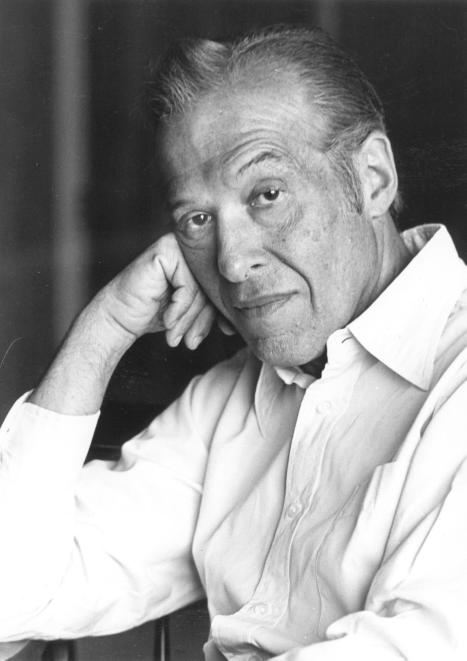
\includegraphics[scale=.35]{./Images/schwinger}
   \caption{Julian Seymour Schwinger (February 12, 1918 -- July 16, 1994) }
\end{figure}

\printbibliography[heading=subbibliography]
\end{refsection}
